%----------------------------------------------------------------------------------------
%	PACKAGES AND THEMES
%----------------------------------------------------------------------------------------
\documentclass[aspectratio=169,xcolor=dvipsnames]{beamer}
\usetheme{SimplePlus}

\usepackage{graphicx}
\usepackage{algorithm2e}
\usepackage{algorithmic}
\usepackage{float}
\usepackage{verbatim}
\usepackage{pgfplots}
\usepackage{tikz}
\usepackage{qrcode}
\usepackage{hyperref}
\newcommand{\mathcolorbox}[2]{\colorbox{#1}{$\displaystyle #2$}}
\usepackage{graphicx} % Allows including images
\usepackage{booktabs} % Allows the use of \toprule, \midrule and \bottomrule in tables

%----------------------------------------------------------------------------------------
%	TITLE PAGE
%----------------------------------------------------------------------------------------

\title[short title]{Advanced Dynamic Programming} % The short title appears at the bottom of every slide, the full title is only on the title page
\subtitle{IPST 2}

\author[Pin-Yen] {Pongsaphol Pongsawakul}


\date{} % Date, can be changed to a custom date


%----------------------------------------------------------------------------------------
%	PRESENTATION SLIDES
%----------------------------------------------------------------------------------------

\begin{document}

\begin{frame}[plain]
    % Print the title page as the first slide
    \titlepage
\end{frame}

\begin{frame}[plain]{Overview}
    % Throughout your presentation, if you choose to use \section{} and \subsection{} commands, these will automatically be printed on this slide as an overview of your presentation
    \tableofcontents
\end{frame}

%------------------------------------------------
\section{Convex Hull Optimization}
%------------------------------------------------

\begin{frame}[plain]{Convex hull optimization}
    \begin{itemize}
        \begin{block}{Equation}
        $dp(i) = \displaystyle\min_{j<i}\{dp(j)+B(j)\cdot A(i)\}$ which $B(j) \geq B(j+1)$ and $A(i) \leq A(i+1)$
        \end{block}
        \item<2-> We want to optimize from $O(n^2)$ to $O(n)$
        \item<3-> $dp(j)+B(j)\cdot A(i)$
        \item<3-> $B(j)\cdot A(i) + dp(j)$
        \item<4-> $f(x) = mx+c$ where $m = B(j)$, $x = A(i)$, $c = dp(j)$
        \item<5-> $B$ is an non-increasing sequence and $A$ is an non-decreasing sequence
    \end{itemize}
\end{frame}

\begin{frame}[plain]{Convex hull optimization}

    \begin{block}{Theorem}
    Let $f_j(x) = m_jx + c_j = B(j)x + dp(j)$ where $m_j = B_j$ and $c_j = dp(j)$
        
    We can re-write $dp(i)$ as $dp(i) = \displaystyle\min_{j<i}\{f_j(x)\}$
    \end{block}
\end{frame}

\begin{frame}[plain]{Convex hull optimization}
    \begin{itemize}
        \item This is a geometry problem
        \item Convex Hull
    \end{itemize}
\end{frame}

\begin{frame}[plain]{Convex hull optimization}

\end{frame}

\begin{frame}[plain]{Convex hull optimization}
    \begin{itemize}
        \item Let $V = \{(m_1, c_1), (m_2, c_2), ..., (m_{i-1}, c_{i-1})\}$
        \item When we want to insert $(m_i, c_i)$ into $V$
        \item We have to check $x_{1} \leq x_2$
    \end{itemize}
\end{frame}

\begin{frame}[plain]{Convex hull optimization}
    \begin{itemize}
        \item<1-> There are 3 lines that we have to check
        \begin{itemize}
            \item $y = m_1x+c_1$
            \item $y = m_2x+c_2$
            \item $y = m_nx+c_n$
        \end{itemize}
        \item<2-> We will get the intersection points
        \begin{itemize}
            \item $x_1 = \frac{c_n-c_1}{m_1-m_n}$
            \item $x_2 = \frac{c_n-c_2}{m_2-m_n}$
        \end{itemize}
        \item<3-> We have to check $x_{1} \leq x_2$
        \begin{itemize}
            \item $\frac{c_n-c_1}{m_1-m_n} \leq \frac{c_n-c_2}{m_2-m_n}$
            \item $(c_n-c_1)(m_2-m_n) \leq (c_n-c_2)(m_1-m_n)$
            \item $(c_n-c_1)(m_2-m_n) - (c_n-c_2)(m_1-m_n) \leq 0$
        \end{itemize}
    \end{itemize}
\end{frame}

\begin{frame}[fragile, plain]{Convex hull optimization}
\begin{examples}
\begin{verbatim}
Algorithm check(y1, y2, yn):
    return (yn.c - y1.c)(y2.m - yn.m) - (yn.c - y2.c)(y1.m - yn.m)

Algorithm AddLine(newline):  // Input: line with attribute m, c
    while V.size >= 2 and check(V.back, V.back.back, newline) <= 0:
        V.pop_back
    while !V.empty and V.back.m == newline.m and V.back.c >= newline.c:
        V.pop_back
    V.push_back(newline)
\end{verbatim}
\end{examples}
\end{frame}

\begin{frame}[fragile, plain]{Convex hull optimization}
\begin{itemize}
    \item How can we get $\displaystyle\min_{j<i}\{f_j(x)\}$
    \item $x = A(i)$ and $A$ is an non-decreasing sequence
\end{itemize}

\end{frame}

\begin{frame}[fragile, plain]{Convex hull optimization}
\end{frame}

\begin{frame}[fragile, plain]{Convex hull optimization}
\begin{examples}
\begin{verbatim}
Algorithm get(ptr, x):
    return V[ptr].m * x + V[ptr].c
ptr = 0
Algorithm query(x):
    if ptr >= vec.size:
        ptr = vec.size - 1
    while ptr + 1 < vec.size and get(ptr, x) >= get(ptr+1, x):
        ptr++
    return get(ptr, x)
\end{verbatim}
\end{examples}

\end{frame}

%------------------------------------------------
\section{Li Chao Tree}
\begin{frame}[plain]{Li Chao Tree}
\begin{block}{Equation}
    $dp(i) = \displaystyle\min_{j<i}\{dp(j)+B(j)\cdot A(i)\}$
\end{block}
\end{frame}

\begin{frame}[plain]{Li Chao Tree}
\begin{itemize}
    \item Use concepts from segment tree to collect lines
    \item time travel (Persistent Li Chao Tree)
\end{itemize}
\end{frame}

\begin{frame}[t, plain]{Li Chao Tree}
\begin{itemize}
    \item In each node, instead of collecting a number, we would collect $(m, c)$ representing a line
    
\end{itemize}
\end{frame}

\begin{frame}[t, plain]{Li Chao Tree}
\begin{itemize}
    \item There are 4 cases that we have to consider
\end{itemize}
\end{frame}

\begin{frame}[t, plain]{Li Chao Tree}
Case \#1:
\begin{center}
\begin{tikzpicture}
\draw (0,0) -- (12,0) -- (12,5) -- (0,5) -- (0,0);
\draw[blue] (0,3) -- (12,2);
\draw[red] (0, 4) -- (12, 5);
\end{tikzpicture}
\end{center}
\end{frame}

\begin{frame}[t, plain]{Li Chao Tree}
Case \#2:

\begin{center}
\begin{tikzpicture}
\draw (0,0) -- (12,0) -- (12,5) -- (0,5) -- (0,0);
\draw[blue] (0,3) -- (12,4);
\draw[red] (0, 2) -- (12, 1);
\end{tikzpicture}
\end{center}
\end{frame}

\begin{frame}[t, plain]{Li Chao Tree}
Case \#3:

\begin{center}
\begin{tikzpicture}
\draw (0,0) -- (12,0) -- (12,5) -- (0,5) -- (0,0);
\draw (6, 0) -- (6, 5);
\draw[red] (0,3) -- (12,4);
\draw[blue] (0, 4) -- (12, 1);
\end{tikzpicture}
\end{center}
\end{frame}

\begin{frame}[t, plain]{Li Chao Tree}
Case \#4:

\begin{center}
\begin{tikzpicture}
\draw (0,0) -- (12,0) -- (12,5) -- (0,5) -- (0,0);
\draw (6, 0) -- (6, 5);
\draw[blue] (0,4) -- (12,3);
\draw[red] (0,1) -- (12, 4);
\end{tikzpicture}
\end{center}
\end{frame}

\begin{frame}[plain, fragile]{Li Chao Tree}
\begin{examples}
\begin{scriptsize}
\begin{verbatim}
Algorithm f(line, x):
    return line.m * x + line.c
    
Algorithm update(newline, p, l, r): 
    if f(newline, l) >= f(node[p], l) and f(newline, r) >= f(node[p], r):
        return // Case 1
    if f(newline, l) <= f(node[p], l) and f(newline, r) <= f(node[p], r):
        swap(newline, node[p]) // Case 2
        return
    // forced f(newline, l) to be less than f(node[p], l)
    if f(newline, l) > f(node[p], l):
        swap(newline, node[p])
    if l == r:
        return
    let m = (l + r) / 2;
    if f(newline, m) > f(node[p], m):
        update(newline, 2*p, l, m) // Case 3
    else:
        swap(newline, node[p])
        update(newline, 2*p + 1, m + 1, r) // Case 4
\end{verbatim}
\end{scriptsize}
\end{examples}
\end{frame}

\begin{frame}[plain, fragile]{Li Chao Tree}
\begin{examples}
\begin{scriptsize}
\begin{verbatim}
Algorithm query(x, p, l, r): 
    let result = f(node[p], x)
    let m = (l + r) / 2
    if x <= m:
        return min(result, query(x, p*2, l, m))
    else:
        return min(result, query(x, p*2 + 1, m + 1, r))
\end{verbatim}
\end{scriptsize}
\end{examples}
\end{frame}

\begin{frame}[plain, fragile]{Li Chao Tree}

\begin{center}
{\large Squared Ends: CSAcademy}

\qrcode[height=2in]{https://csacademy.com/contest/archive/task/squared-ends}
\end{center}
\end{frame}

\begin{frame}[t, plain, fragile]{Li Chao Tree}
You are given an array $A$ of $N$ integers. The cost of a subarray $[A_l, A_{l+1}, ..., A_r]$ is equal to $(A_l - A_r)^2$. Partition the array in $K$ subarrays having a minimum total cost.
\begin{itemize}
    \item $1 \leq N \leq 10^4$
    \item $1 \leq K \leq \min(N, 100)$
    \item $1 \leq A_i \leq 10^6$
    \item Time limit: 2000 ms
    \item Memory limit: 256 MB
\end{itemize}
\end{frame}

\begin{frame}[t, plain, fragile]{Li Chao Tree}
You are given an array $A$ of $N$ integers. The cost of a subarray $[A_l, A_{l+1}, ..., A_r]$ is equal to $(A_l - A_r)^2$. Partition the array in $K$ subarrays having a minimum total cost.
\begin{itemize}
    \item We know that $(A_l - A_r)^2 = A_l^2 - 2A_lA_r + A_r^2$
    \pause
    \item Let $cost(l, r) = (A_l - A_r)^2 = A_l^2 - 2A_lA_r + A_r^2$
    \pause
    \item Let $dp(i, j)$ be the minimum total cost when there are $i$ partitions and we consider only $A_1, ..., A_j$.
    \pause
    \item $dp(i, j) = \displaystyle\min_{i\leq k\leq j}\{dp(i-1, k-1) + cost(k, j)\}$
    \pause
    \item $dp(i, j) = \displaystyle\min_{i\leq k\leq j}\{dp(i-1, k-1) + A_k^2 - 2A_kA_j + A_j^2\}$
    \pause
    \item $dp(i, j) = \displaystyle\min_{i\leq k\leq j}\{(-2A_k)A_j + (dp(i-1, k-1) + A_k^2)\} + A_j^2$
\end{itemize}
\end{frame}

\begin{frame}[t, plain, fragile]{Li Chao Tree}
You are given an array $A$ of $N$ integers. The cost of a subarray $[A_l, A_{l+1}, ..., A_r]$ is equal to $(A_l - A_r)^2$. Partition the array in $K$ subarrays having a minimum total cost.
\begin{itemize}
    \item $dp(i, j) = \displaystyle\min_{i\leq k\leq j}\{(-2A_k)A_j + (dp(i-1, k-1) + A_k^2)\} + A_j^2$
    \pause
    \item $m = (-2A_k)$ and $c = dp(i-1, k-1) + A_k^2$
\end{itemize}
\end{frame}

\begin{frame}[t, plain, fragile]{Li Chao Tree}
You are given an array $A$ of $N$ integers. The cost of a subarray $[A_l, A_{l+1}, ..., A_r]$ is equal to $(A_l - A_r)^2$. Partition the array in $K$ subarrays having a minimum total cost.
\begin{itemize}
    \item $dp(i, j) = \displaystyle\min_{i\leq k\leq j}\{(-2A_k)A_j + (dp(i-1, k-1) + A_k^2)\} + A_j^2$
\end{itemize}
\begin{block}{Solution}
\begin{verbatim}
Algorithm solve(A[1..N], K): 
    for i in 1...N:
        dp(1, i) = (A[1] - A[i])^2
    for i in 2...K:
        for j in i...N:
            update((-2A[j], A[j]^2 + dp(i-1, j-1))
            dp(i, j) = query(A[j]) + A[j]^2
        clear_tree()
    return dp(K, N)
\end{verbatim}
\end{block}
\end{frame}



%------------------------------------------------
\section{Slope Trick}
\begin{frame}[t, plain]{Slope Trick}
\begin{itemize}
    \item Finding $\min\{|A_1 - x| + |A_2 - x| + ... + |A_n - x|\}$
    \pause
    \item Plot a graph
\end{itemize}
\end{frame}

\begin{frame}[t, plain]{Slope Trick}
What do we need to collect in the data structure?
\pause
\begin{itemize}
    \item $y$, y-intersect
    \pause 
    \item $m$, the initial slope
    \pause
    \item slope change points (We can collect them in \texttt{std::multiset} or \texttt{std::vector}), called $S$
    \pause
    \item We also call this data structure $D$
\end{itemize}
\end{frame}

\begin{frame}[t, plain]{Slope Trick}
We have a merge operation
\pause
\begin{examples}
We want to merge $D_1$ and $D_2$ collected in $D'$
\pause
\begin{itemize}
    \item $y' = y_1 + y_2$
    \pause 
    \item $m' = m_1 + m_2$
    \pause
    \item $S' = S_1 + S_2$
\end{itemize}
\end{examples}
\end{frame}

\begin{frame}[t, plain]{Slope Trick}
We can use this concept to apply with
\pause
\begin{itemize}
    \item merge small into large
    \pause
    \item lazy set
\end{itemize}

\end{frame}

\begin{frame}[t, plain]{Slope Trick}
\begin{Large}
NOI2019 - Safety
\end{Large}
\begin{columns}[c] % The "c" option specifies centered vertical alignment while the "t" option is used for top vertical alignment

        \column{.45\textwidth} % Left column and width
        \begin{alertblock}{Example Input}
\texttt{6 1}

\texttt{2 10 0 2 4 3}
\end{alertblock}
        \column{.45\textwidth} % Right column and width
        \begin{alertblock}{Example Output}
\texttt{10}

\texttt{}
\end{alertblock}
\end{columns}

\begin{center}
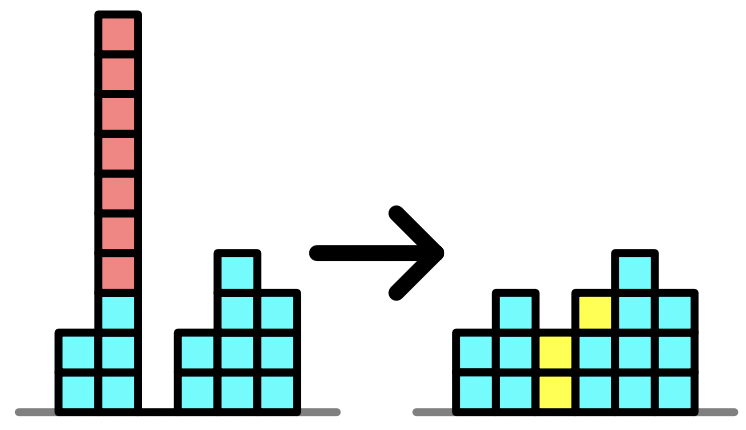
\includegraphics[width=6.5cm]{safety.png}
\end{center}

\end{frame}

\begin{frame}[t, plain]{Slope Trick}
\begin{columns}[c]
\column{.45\textwidth}
\begin{gather*}
H = 1,S = \{\mathcolorbox{yellow}{2}, 10, 0, 2, 4, 3\}
\end{gather*}
\column{.45\textwidth}
\begin{gather*}
y_{min} = 0,D = \{\mathcolorbox{yellow}{2, 2}\}
\end{gather*}
\end{columns}

\begin{center}
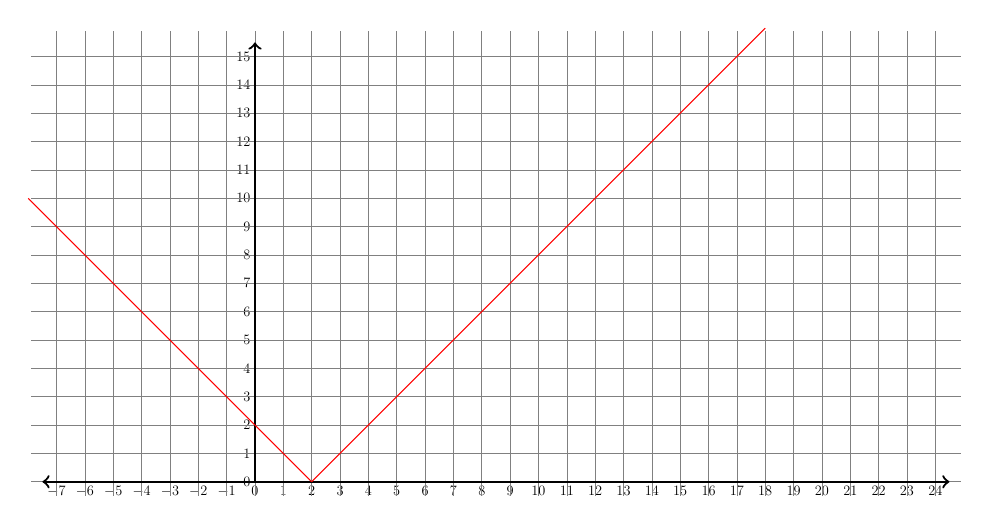
\begin{tikzpicture}[scale=0.36, transform shape]
    \foreach \x in {-7,-6,-5,-4,-3,-2,-1,0,1,2,3,4,5,6,7,8,9,10,11,12,13,14,15,16,17,18,19,20,21,22,23,24}
        \draw (\x cm,1pt) -- (\x cm,-1pt) node[anchor=north] {\Large $\x$};
    \foreach \y in {0,1,2,3,4,5,6,7,8,9,10,11,12,13,14,15}
        \draw (1pt,\y cm) -- (-1pt,\y cm) node[anchor=east] {\Large $\y$};
    \draw[step=1cm,gray,very thin] (-7.9,-0.5) grid (24.9,15.9);
    \draw[thick,<->] (-7.5,0) -- (24.5,0);
    \draw[thick,->] (0,0) -- (0,15.5);
    
    \draw[red] (2,0) -- (-8, 10);
    \draw[red] (2,0) -- (18, 16);
    % \node [left] at (0,1) {$1$};                % label y-intercept
    % \node [below] at (1,0) {$1$};               % label x-intercept
\end{tikzpicture}
\end{center}
\end{frame}

\begin{frame}[t, plain]{Slope Trick}
\begin{columns}[c]
\column{.45\textwidth}
\begin{gather*}
H = 1,S = \{2, 10, 0, 2, 4, 3\}
\end{gather*}
\column{.45\textwidth}
\begin{gather*}
y_{min} = 0,D = \{1, 3\}
\end{gather*}
\end{columns}

\begin{center}
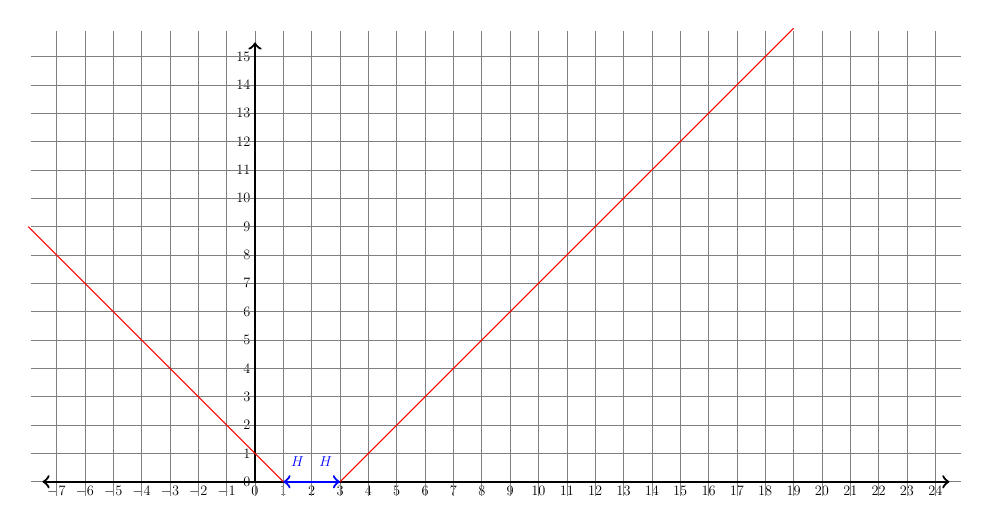
\begin{tikzpicture}[scale=0.36, transform shape]
    \foreach \x in {-7,-6,-5,-4,-3,-2,-1,0,1,2,3,4,5,6,7,8,9,10,11,12,13,14,15,16,17,18,19,20,21,22,23,24}
        \draw (\x cm,1pt) -- (\x cm,-1pt) node[anchor=north] {\Large $\x$};
    \foreach \y in {0,1,2,3,4,5,6,7,8,9,10,11,12,13,14,15}
        \draw (1pt,\y cm) -- (-1pt,\y cm) node[anchor=east] {\Large $\y$};
    \draw[step=1cm,gray,very thin] (-7.9,-0.5) grid (24.9,15.9);
    \draw[thick,<->] (-7.5,0) -- (24.5,0);
    \draw[thick,->] (0,0) -- (0,15.5);
    
    \draw[red] (1,0) -- (-8, 9);
    \draw[red] (1,0) -- (3,0);
    \draw[red] (3,0) -- (19, 16);
    \pause
    \draw[blue,thick,<-] (1,0) -- (2,0);
    \node [blue,below] at (1.5,1) {\Large $H$};
    \draw[blue,thick,->] (2,0) -- (3,0);
    \node [blue,below] at (2.5,1) {\Large $H$}; 
\end{tikzpicture}
\end{center}
\end{frame}

\begin{frame}[t, plain]{Slope Trick}
\begin{columns}[c]
\column{.45\textwidth}
\begin{gather*}
H = 1,S = \{2, 10, 0, 2, 4, 3\}
\end{gather*}
\column{.45\textwidth}
\begin{gather*}
y_{min} = 0,D = \{1, 3\}
\end{gather*}
\end{columns}

\begin{center}
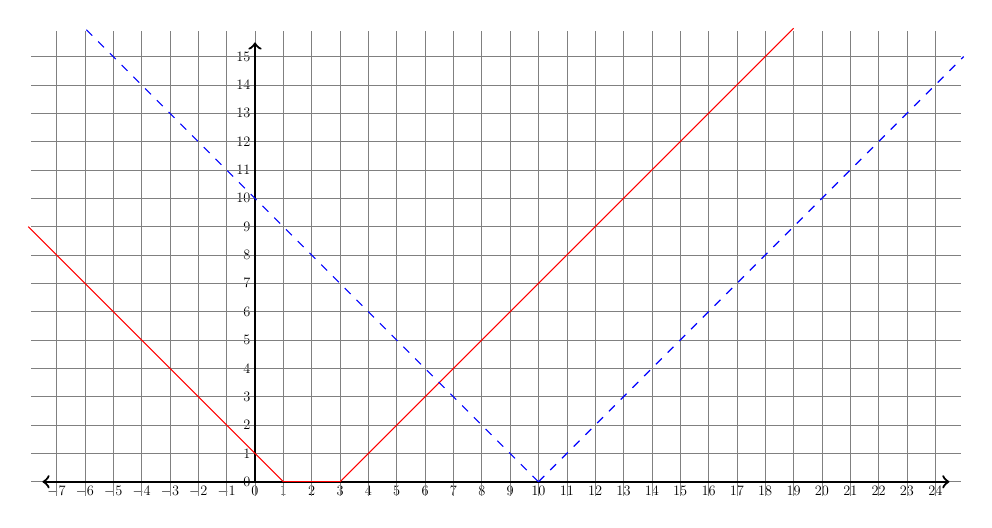
\begin{tikzpicture}[scale=0.36, transform shape]
    \foreach \x in {-7,-6,-5,-4,-3,-2,-1,0,1,2,3,4,5,6,7,8,9,10,11,12,13,14,15,16,17,18,19,20,21,22,23,24}
        \draw (\x cm,1pt) -- (\x cm,-1pt) node[anchor=north] {\Large $\x$};
    \foreach \y in {0,1,2,3,4,5,6,7,8,9,10,11,12,13,14,15}
        \draw (1pt,\y cm) -- (-1pt,\y cm) node[anchor=east] {\Large $\y$};
    \draw[step=1cm,gray,very thin] (-7.9,-0.5) grid (24.9,15.9);
    \draw[thick,<->] (-7.5,0) -- (24.5,0);
    \draw[thick,->] (0,0) -- (0,15.5);
    
    \draw[red] (1,0) -- (-8, 9);
    \draw[red] (1,0) -- (3,0);
    \draw[red] (3,0) -- (19, 16);
    \pause
    \draw[blue, dashed] (10, 0) -- (-6,16);
    \draw[blue, dashed] (10, 0) -- (25,15);
\end{tikzpicture}
\end{center}
\end{frame}

\begin{frame}[t, plain]{Slope Trick}
\begin{columns}[c]
\column{.45\textwidth}
\begin{gather*}
H = 1,S = \{2,\mathcolorbox{yellow}{10}, 0, 2, 4, 3\}
\end{gather*}
\column{.45\textwidth}
\begin{gather*}
y_{min} = 7,D = \{1, 3, 10, 10\}
\end{gather*}
\end{columns}

\begin{center}
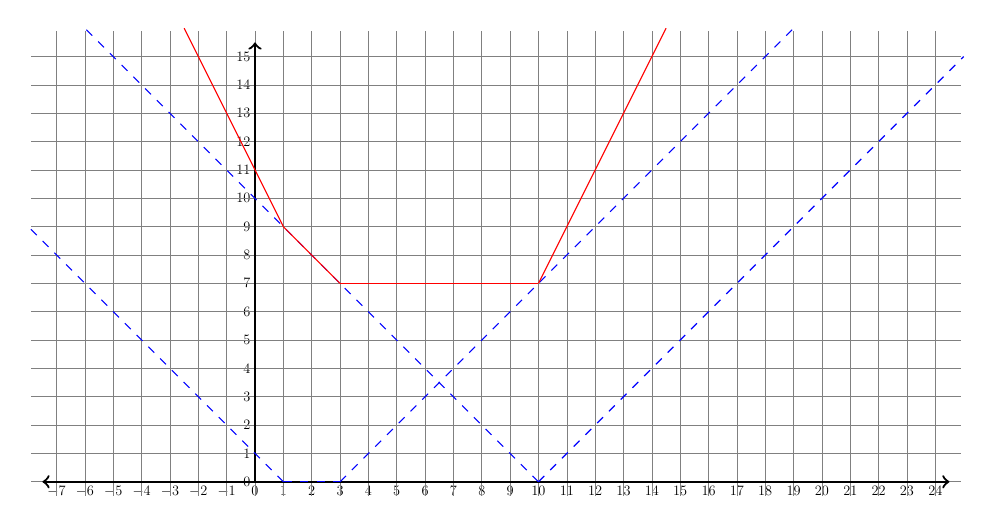
\begin{tikzpicture}[scale=0.36, transform shape]
    \foreach \x in {-7,-6,-5,-4,-3,-2,-1,0,1,2,3,4,5,6,7,8,9,10,11,12,13,14,15,16,17,18,19,20,21,22,23,24}
        \draw (\x cm,1pt) -- (\x cm,-1pt) node[anchor=north] {\Large $\x$};
    \foreach \y in {0,1,2,3,4,5,6,7,8,9,10,11,12,13,14,15}
        \draw (1pt,\y cm) -- (-1pt,\y cm) node[anchor=east] {\Large $\y$};
    \draw[step=1cm,gray,very thin] (-7.9,-0.5) grid (24.9,15.9);
    \draw[thick,<->] (-7.5,0) -- (24.5,0);
    \draw[thick,->] (0,0) -- (0,15.5);
    
    \draw[blue, dashed] (1,0) -- (-8, 9);
    \draw[blue, dashed] (1,0) -- (3,0);
    \draw[blue, dashed] (3,0) -- (19, 16);
    \pause
    \draw[blue, dashed] (10, 0) -- (-6,16);
    \draw[blue, dashed] (10, 0) -- (25,15);
    \pause
    \draw[red] (3,7) -- (10,7);
    \draw[red] (10,7) -- (14.5,16);
    \draw[red] (3,7) -- (1,9);
    \draw[red] (1,9) -- (-2.5,16);
\end{tikzpicture}
\end{center}
\end{frame}

\begin{frame}[t, plain]{Slope Trick}
\begin{columns}[c]
\column{.45\textwidth}
\begin{gather*}
H = 1,S = \{2,10, 0, 2, 4, 3\}
\end{gather*}
\column{.45\textwidth}
\begin{gather*}
y_{min} = 7,D = \{0, 2, 11, 11\}
\end{gather*}
\end{columns}

\begin{center}
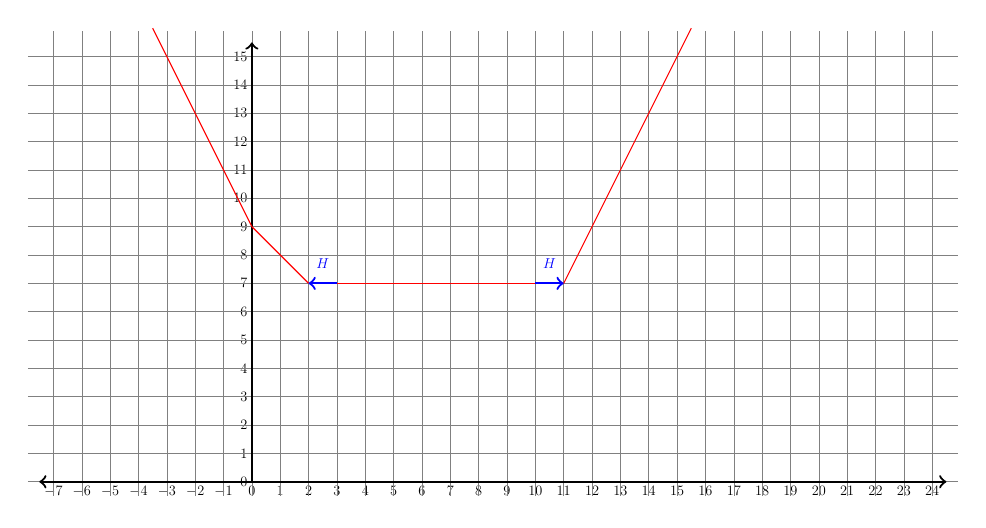
\begin{tikzpicture}[scale=0.36, transform shape]
    \foreach \x in {-7,-6,-5,-4,-3,-2,-1,0,1,2,3,4,5,6,7,8,9,10,11,12,13,14,15,16,17,18,19,20,21,22,23,24}
        \draw (\x cm,1pt) -- (\x cm,-1pt) node[anchor=north] {\Large $\x$};
    \foreach \y in {0,1,2,3,4,5,6,7,8,9,10,11,12,13,14,15}
        \draw (1pt,\y cm) -- (-1pt,\y cm) node[anchor=east] {\Large $\y$};
    \draw[step=1cm,gray,very thin] (-7.9,-0.5) grid (24.9,15.9);
    \draw[thick,<->] (-7.5,0) -- (24.5,0);
    \draw[thick,->] (0,0) -- (0,15.5);
    \draw[red] (2,7) -- (11,7);
    \draw[red] (11,7) -- (15.5,16);
    \draw[red] (2,7) -- (0,9);
    \draw[red] (0,9) -- (-3.5,16);
    \draw[blue,thick,<-] (2,7) -- (3,7);
    \node [blue,below] at (2.5,8) {\Large $H$};
    \draw[blue,thick,->] (10,7) -- (11,7);
    \node [blue,below] at (10.5,8) {\Large $H$}; 
\end{tikzpicture}
\end{center}
\end{frame}

\begin{frame}[t, plain]{Slope Trick}
\begin{columns}[c]
\column{.45\textwidth}
\begin{gather*}
H = 1,S = \{2, 10, \mathcolorbox{yellow}{0}, 2, 4, 3\}
\end{gather*}
\column{.45\textwidth}
\begin{gather*}
y_{min} = 7,D = \{0, 2, 11, 11\}
\end{gather*}
\end{columns}
\begin{center}
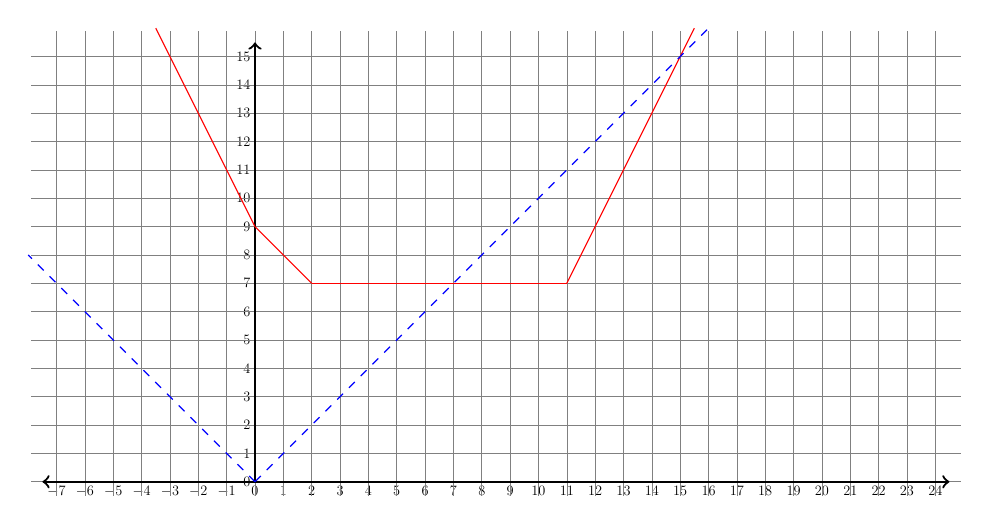
\begin{tikzpicture}[scale=0.36, transform shape]
    \foreach \x in {-7,-6,-5,-4,-3,-2,-1,0,1,2,3,4,5,6,7,8,9,10,11,12,13,14,15,16,17,18,19,20,21,22,23,24}
        \draw (\x cm,1pt) -- (\x cm,-1pt) node[anchor=north] {\Large $\x$};
    \foreach \y in {0,1,2,3,4,5,6,7,8,9,10,11,12,13,14,15}
        \draw (1pt,\y cm) -- (-1pt,\y cm) node[anchor=east] {\Large $\y$};
    \draw[step=1cm,gray,very thin] (-7.9,-0.5) grid (24.9,15.9);
    \draw[thick,<->] (-7.5,0) -- (24.5,0);
    \draw[thick,->] (0,0) -- (0,15.5);
    \draw[red] (2,7) -- (11,7);
    \draw[red] (11,7) -- (15.5,16);
    \draw[red] (2,7) -- (0,9);
    \draw[red] (0,9) -- (-3.5,16);
    \draw[blue, dashed] (0,0) -- (-8,8);
    \draw[blue, dashed] (0,0) -- (16,16);
\end{tikzpicture}
\end{center}
\end{frame}

\begin{frame}[t, plain]{Slope Trick}
\begin{columns}[c]
\column{.45\textwidth}
\begin{gather*}
H = 1,S = \{2, 10, \mathcolorbox{yellow}{0}, 2, 4, 3\}
\end{gather*}
\column{.45\textwidth}
\begin{gather*}
y_{min} = 9,D = \{0, 0, 0, 2, 11, 11\}
\end{gather*}
\end{columns}
\begin{center}
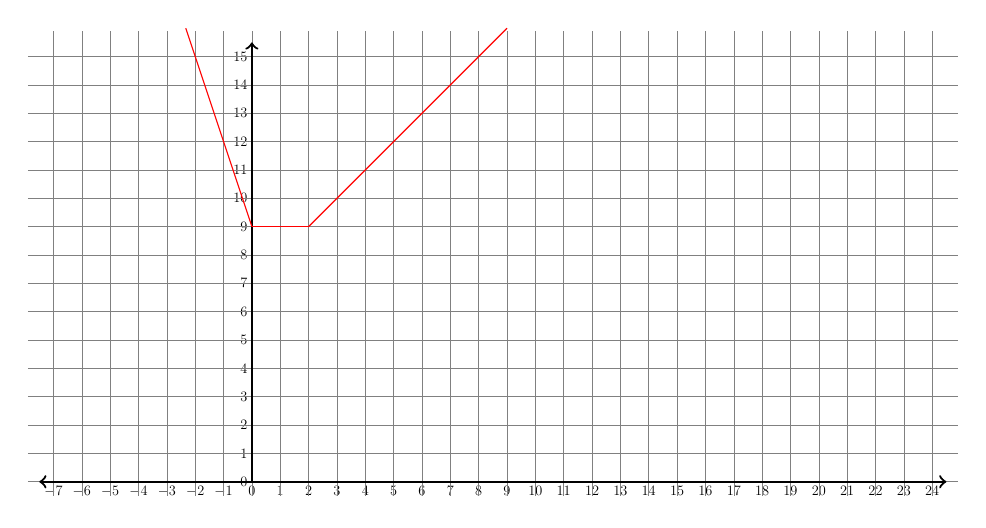
\begin{tikzpicture}[scale=0.36, transform shape]
    \foreach \x in {-7,-6,-5,-4,-3,-2,-1,0,1,2,3,4,5,6,7,8,9,10,11,12,13,14,15,16,17,18,19,20,21,22,23,24}
        \draw (\x cm,1pt) -- (\x cm,-1pt) node[anchor=north] {\Large $\x$};
    \foreach \y in {0,1,2,3,4,5,6,7,8,9,10,11,12,13,14,15}
        \draw (1pt,\y cm) -- (-1pt,\y cm) node[anchor=east] {\Large $\y$};
    \draw[step=1cm,gray,very thin] (-7.9,-0.5) grid (24.9,15.9);
    \draw[thick,<->] (-7.5,0) -- (24.5,0);
    \draw[thick,->] (0,0) -- (0,15.5);
    \draw[red] (0, 9) -- (2, 9);
    \draw[red] (0, 9) -- (-2.333, 16);
    \draw[red] (2, 9) -- (9, 16);
\end{tikzpicture}
\end{center}
\end{frame}

\begin{frame}[t, plain]{Slope Trick}
\begin{columns}[c]
\column{.35\textwidth}
\begin{gather*}
H = 1,S = \{2, 10, 0, 2, 4, \mathcolorbox{yellow}{3}\}
\end{gather*}
\column{.60\textwidth}
\begin{gather*}
y_{min} = 10,D = \{-3,-3,-3,0,2,3,3,5,5,5,14,14\}
\end{gather*}
\end{columns}
\begin{center}
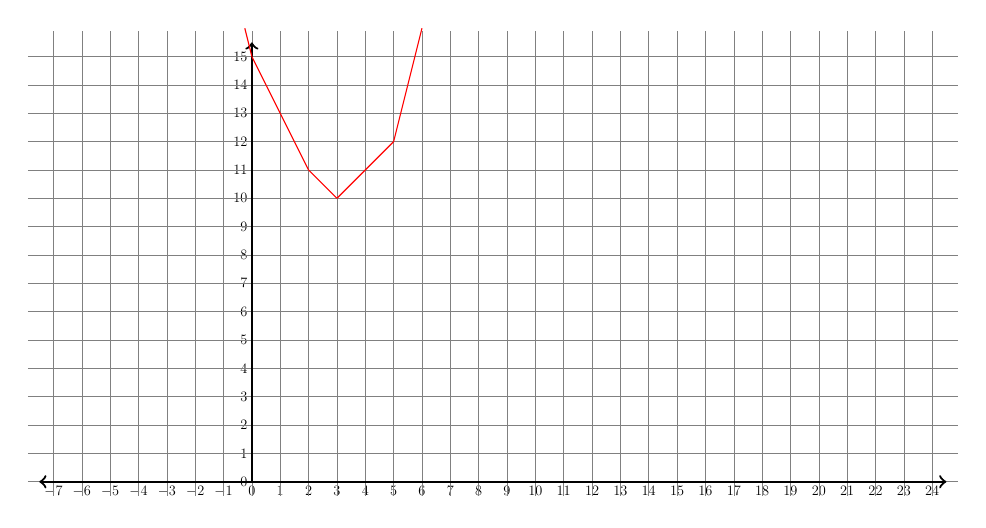
\begin{tikzpicture}[scale=0.36, transform shape]
    \foreach \x in {-7,-6,-5,-4,-3,-2,-1,0,1,2,3,4,5,6,7,8,9,10,11,12,13,14,15,16,17,18,19,20,21,22,23,24}
        \draw (\x cm,1pt) -- (\x cm,-1pt) node[anchor=north] {\Large $\x$};
    \foreach \y in {0,1,2,3,4,5,6,7,8,9,10,11,12,13,14,15}
        \draw (1pt,\y cm) -- (-1pt,\y cm) node[anchor=east] {\Large $\y$};
    \draw[step=1cm,gray,very thin] (-7.9,-0.5) grid (24.9,15.9);
    \draw[thick,<->] (-7.5,0) -- (24.5,0);
    \draw[thick,->] (0,0) -- (0,15.5);
    \draw[red] (3, 10) -- (5, 12);
    \draw[red] (5, 12) -- (6, 16);
    \draw[red] (3, 10) -- (2, 11);
    \draw[red] (2, 11) -- (0, 15);
    \draw[red] (0, 15) -- (-0.25, 16);
\end{tikzpicture}
\end{center}
\end{frame}

%------------------------------------------------

\section{Divide and Conquer Optimization}
\begin{frame}[plain]{Divide and Conquer Optimization}
\end{frame}
\section{Knuth Optimization}
\begin{frame}[plain]{Knuth Optimization}
\end{frame}
\section{Open and Close Interval Trick}
\begin{frame}[plain]{Open and Close Interval Trick}
\end{frame}
\section{Connected Component DP}
\begin{frame}[plain]{Connected Component DP}
\end{frame}
\section{Sum of Subset DP}
\begin{frame}[plain]{Sum of Subset DP}
\end{frame}
\end{document}